% Options for packages loaded elsewhere
\PassOptionsToPackage{unicode}{hyperref}
\PassOptionsToPackage{hyphens}{url}
\PassOptionsToPackage{dvipsnames,svgnames,x11names}{xcolor}
%
\documentclass[
  10pt,
]{article}
\usepackage{amsmath,amssymb}
\usepackage{iftex}
\ifPDFTeX
  \usepackage[T1]{fontenc}
  \usepackage[utf8]{inputenc}
  \usepackage{textcomp} % provide euro and other symbols
\else % if luatex or xetex
  \usepackage{unicode-math} % this also loads fontspec
  \defaultfontfeatures{Scale=MatchLowercase}
  \defaultfontfeatures[\rmfamily]{Ligatures=TeX,Scale=1}
\fi
\usepackage{lmodern}
\ifPDFTeX\else
  % xetex/luatex font selection
  \setmainfont[]{DejaVu Serif}
  \setsansfont[]{DejaVu Sans}
  \setmonofont[]{DejaVu Sans Mono}
  \setmathfont[]{Latin Modern Math}
\fi
% Use upquote if available, for straight quotes in verbatim environments
\IfFileExists{upquote.sty}{\usepackage{upquote}}{}
\IfFileExists{microtype.sty}{% use microtype if available
  \usepackage[]{microtype}
  \UseMicrotypeSet[protrusion]{basicmath} % disable protrusion for tt fonts
}{}
\makeatletter
\@ifundefined{KOMAClassName}{% if non-KOMA class
  \IfFileExists{parskip.sty}{%
    \usepackage{parskip}
  }{% else
    \setlength{\parindent}{0pt}
    \setlength{\parskip}{6pt plus 2pt minus 1pt}}
}{% if KOMA class
  \KOMAoptions{parskip=half}}
\makeatother
\usepackage{xcolor}
\usepackage[margin=2.0cm]{geometry}
\usepackage{color}
\usepackage{fancyvrb}
\newcommand{\VerbBar}{|}
\newcommand{\VERB}{\Verb[commandchars=\\\{\}]}
\DefineVerbatimEnvironment{Highlighting}{Verbatim}{commandchars=\\\{\}}
% Add ',fontsize=\small' for more characters per line
\newenvironment{Shaded}{}{}
\newcommand{\AlertTok}[1]{\textcolor[rgb]{1.00,0.00,0.00}{\textbf{#1}}}
\newcommand{\AnnotationTok}[1]{\textcolor[rgb]{0.38,0.63,0.69}{\textbf{\textit{#1}}}}
\newcommand{\AttributeTok}[1]{\textcolor[rgb]{0.49,0.56,0.16}{#1}}
\newcommand{\BaseNTok}[1]{\textcolor[rgb]{0.25,0.63,0.44}{#1}}
\newcommand{\BuiltInTok}[1]{\textcolor[rgb]{0.00,0.50,0.00}{#1}}
\newcommand{\CharTok}[1]{\textcolor[rgb]{0.25,0.44,0.63}{#1}}
\newcommand{\CommentTok}[1]{\textcolor[rgb]{0.38,0.63,0.69}{\textit{#1}}}
\newcommand{\CommentVarTok}[1]{\textcolor[rgb]{0.38,0.63,0.69}{\textbf{\textit{#1}}}}
\newcommand{\ConstantTok}[1]{\textcolor[rgb]{0.53,0.00,0.00}{#1}}
\newcommand{\ControlFlowTok}[1]{\textcolor[rgb]{0.00,0.44,0.13}{\textbf{#1}}}
\newcommand{\DataTypeTok}[1]{\textcolor[rgb]{0.56,0.13,0.00}{#1}}
\newcommand{\DecValTok}[1]{\textcolor[rgb]{0.25,0.63,0.44}{#1}}
\newcommand{\DocumentationTok}[1]{\textcolor[rgb]{0.73,0.13,0.13}{\textit{#1}}}
\newcommand{\ErrorTok}[1]{\textcolor[rgb]{1.00,0.00,0.00}{\textbf{#1}}}
\newcommand{\ExtensionTok}[1]{#1}
\newcommand{\FloatTok}[1]{\textcolor[rgb]{0.25,0.63,0.44}{#1}}
\newcommand{\FunctionTok}[1]{\textcolor[rgb]{0.02,0.16,0.49}{#1}}
\newcommand{\ImportTok}[1]{\textcolor[rgb]{0.00,0.50,0.00}{\textbf{#1}}}
\newcommand{\InformationTok}[1]{\textcolor[rgb]{0.38,0.63,0.69}{\textbf{\textit{#1}}}}
\newcommand{\KeywordTok}[1]{\textcolor[rgb]{0.00,0.44,0.13}{\textbf{#1}}}
\newcommand{\NormalTok}[1]{#1}
\newcommand{\OperatorTok}[1]{\textcolor[rgb]{0.40,0.40,0.40}{#1}}
\newcommand{\OtherTok}[1]{\textcolor[rgb]{0.00,0.44,0.13}{#1}}
\newcommand{\PreprocessorTok}[1]{\textcolor[rgb]{0.74,0.48,0.00}{#1}}
\newcommand{\RegionMarkerTok}[1]{#1}
\newcommand{\SpecialCharTok}[1]{\textcolor[rgb]{0.25,0.44,0.63}{#1}}
\newcommand{\SpecialStringTok}[1]{\textcolor[rgb]{0.73,0.40,0.53}{#1}}
\newcommand{\StringTok}[1]{\textcolor[rgb]{0.25,0.44,0.63}{#1}}
\newcommand{\VariableTok}[1]{\textcolor[rgb]{0.10,0.09,0.49}{#1}}
\newcommand{\VerbatimStringTok}[1]{\textcolor[rgb]{0.25,0.44,0.63}{#1}}
\newcommand{\WarningTok}[1]{\textcolor[rgb]{0.38,0.63,0.69}{\textbf{\textit{#1}}}}
\usepackage{longtable,booktabs,array}
\usepackage{calc} % for calculating minipage widths
% Correct order of tables after \paragraph or \subparagraph
\usepackage{etoolbox}
\makeatletter
\patchcmd\longtable{\par}{\if@noskipsec\mbox{}\fi\par}{}{}
\makeatother
% Allow footnotes in longtable head/foot
\IfFileExists{footnotehyper.sty}{\usepackage{footnotehyper}}{\usepackage{footnote}}
\makesavenoteenv{longtable}
\usepackage{graphicx}
\makeatletter
\def\maxwidth{\ifdim\Gin@nat@width>\linewidth\linewidth\else\Gin@nat@width\fi}
\def\maxheight{\ifdim\Gin@nat@height>\textheight\textheight\else\Gin@nat@height\fi}
\makeatother
% Scale images if necessary, so that they will not overflow the page
% margins by default, and it is still possible to overwrite the defaults
% using explicit options in \includegraphics[width, height, ...]{}
\setkeys{Gin}{width=\maxwidth,height=\maxheight,keepaspectratio}
% Set default figure placement to htbp
\makeatletter
\def\fps@figure{htbp}
\makeatother
\setlength{\emergencystretch}{3em} % prevent overfull lines
\providecommand{\tightlist}{%
  \setlength{\itemsep}{0pt}\setlength{\parskip}{0pt}}
\setcounter{secnumdepth}{-\maxdimen} % remove section numbering
% doc_header.tex -- LaTeX preamble additions used by build_docs.sh for every
% Markdown -> LaTeX -> PDF conversion (supplements, README, submission files).
\usepackage{etoolbox}
% longtable may not be loaded by pandoc when a document has no table
\usepackage{longtable}
% bold vectors: \bm -> \symbf under unicode-math (XeLaTeX), bm package otherwise
\makeatletter
\@ifpackageloaded{unicode-math}{\providecommand{\bm}[1]{\symbf{#1}}}{\usepackage{bm}}
\makeatother
% smaller type in long tables so that wide audit tables fit the text width;
% inside a table a line break is allowed after an underscore of plain text
% (pandoc writes it as \_), so that long identifiers wrap inside their column
% rows are set a little apart, so that symbols with indices do not touch
\AtBeginEnvironment{longtable}{\footnotesize\renewcommand{\arraystretch}{1.45}%
  \let\sptunderscore\_\def\_{\sptunderscore\allowbreak}}
\setlength{\LTcapwidth}{\textwidth}
% allow line breaks after slashes and hyphens inside table cells
\usepackage{xurl}
% code blocks: break over-long lines instead of running into the margin.
% Plain ``` blocks are typeset by pandoc as {verbatim}, highlighted ones
% (```bash) as {Highlighting}; both are re-declared as breakable fancyvrb
% environments.  The continuation line is marked with a small hooked arrow.
\usepackage{fvextra}
\RecustomVerbatimEnvironment{verbatim}{Verbatim}{breaklines,breakanywhere,fontsize=\small}
\makeatletter
\@ifundefined{Highlighting}{}{%
  \RecustomVerbatimEnvironment{Highlighting}{Verbatim}{breaklines,breakanywhere,fontsize=\small,commandchars=\\\{\}}}
\makeatother
% inline code (pandoc writes it as \texttt{...}): never hyphenate -- an inserted
% hyphen could be read as part of a file name -- but allow a line break after
% an underscore, slash, comma, colon or equals sign, so that long paths and
% column lists wrap inside the text width and inside table columns.
% Inside a formula (e.g. the name of a notebook symbol in an equation) the same
% command must first leave math mode, which \text of amsmath does.
\ExplSyntaxOn
\tl_new:N \l__spt_code_tl
\cs_new_protected:Npn \__spt_texttt:n #1
  {
    \tl_set:Nn \l__spt_code_tl {#1}
    \regex_replace_all:nnN { ([\/\,\:\=]) } { \1 \c{allowbreak} } \l__spt_code_tl
    \regex_replace_all:nnN { \c{_} } { \c{_} \c{allowbreak} } \l__spt_code_tl
    \group_begin: \ttfamily \hyphenchar \font = -1 \scan_stop: \l__spt_code_tl \group_end:
  }
\RenewDocumentCommand \texttt { m }
  {
    \mode_if_math:TF { \text { \__spt_texttt:n {#1} } } { \__spt_texttt:n {#1} }
  }
\ExplSyntaxOff
% A figure is written in the Markdown source as an image paragraph followed by
% a caption paragraph ("**Figure S1.** ..."), so that the caption is also
% visible on GitHub.  An image that starts a paragraph is centered.
\usepackage{graphicx}% pandoc loads it only for documents that contain an image
\NewCommandCopy\sptincludegraphics\includegraphics
\RenewDocumentCommand\includegraphics{O{} m}{%
  \ifvmode\begin{center}\sptincludegraphics[#1]{#2}\end{center}%
  \else\sptincludegraphics[#1]{#2}\fi}
% keep figures where they are referenced
\usepackage{float}
\floatplacement{figure}{H}
% running header with the document title
\usepackage{fancyhdr}
\pagestyle{fancy}
\fancyhf{}
\fancyhead[L]{\small PROJECT spacetimes, Revision\_Deflation --- documentation and provenance}
\fancyhead[R]{\small\thepage}
\renewcommand{\headrulewidth}{0.4pt}
% 16x16 matrices: tighter columns so that a full matrix fits the text width
\setlength{\arraycolsep}{3.2pt}
% The documents of this project contain long tagged symbols, file paths and
% identifiers that cannot be hyphenated.  A paragraph is therefore allowed to
% have looser lines before TeX gives up and lets a line stick out of the margin.
\AtBeginDocument{\tolerance=2000 \emergencystretch=5em \hbadness=2000}
\ifLuaTeX
  \usepackage{selnolig}  % disable illegal ligatures
\fi
\IfFileExists{bookmark.sty}{\usepackage{bookmark}}{\usepackage{hyperref}}
\IfFileExists{xurl.sty}{\usepackage{xurl}}{} % add URL line breaks if available
\urlstyle{same}
\hypersetup{
  pdftitle={RS4 --- The effective action of Cornwall, Jackiw and Tomboulis along the deflation clock},
  pdfauthor={Prepared for Patrick Lee Nash, Ph.D.},
  colorlinks=true,
  linkcolor={blue},
  filecolor={Maroon},
  citecolor={blue},
  urlcolor={blue},
  pdfcreator={LaTeX via pandoc}}

\title{RS4 --- The effective action of Cornwall, Jackiw and Tomboulis
along the deflation clock}
\usepackage{etoolbox}
\makeatletter
\providecommand{\subtitle}[1]{% add subtitle to \maketitle
  \apptocmd{\@title}{\par {\large #1 \par}}{}{}
}
\makeatother
\subtitle{PROJECT spacetimes, Revision\_Deflation. Supplement to both
manuscripts of the revision: the paired state, matter, temperature and
the vacuum of the two models as the couplings grow}
\author{Prepared for Patrick Lee Nash, Ph.D.}
\date{November 12, 2026}

\begin{document}
\maketitle

\hypertarget{purpose-and-summary-of-the-results}{%
\section{0. Purpose, and summary of the
results}\label{purpose-and-summary-of-the-results}}

The supplement S4 of the main project derives the properties of the two
models from one function, the effective action for composite operators
of Cornwall, Jackiw and Tomboulis (CJT): the gap equation of the paired
state is its stationarity condition, the condensation energy is its
value, and the same action gives the fermion mass in matter, its melting
at high temperature, and the stability of the vacuum. S4 does this for
one value of the coupling at a time.

The supplement RS1 of the revision shows that on the deflating
spacetimes the models of the main project hold unchanged for the
weighted fields, with a coupling that grows with the ordinary time:
\(g_{VS}\propto e^{\tau_d/2}\), where
\(\tau_d=\mathrm{gsum}\,(x4-x4_{\rm ref})\) is the deflation clock. This
supplement therefore repeats every calculation of S4 \emph{along the
clock}: at a sequence of moments, each with the coupling of that moment.
The reader needs S4 for the method and RS1, Sec. 1, for the clock. The
results:

\begin{enumerate}
\def\labelenumi{\arabic{enumi}.}
\tightlist
\item
  \textbf{The paired state} (Sec. 2). At every moment the solution of
  the gap equation is a minimum of the CJT potential. The condensation
  energy deepens monotonically, in weak coupling with twice the
  logarithmic slope of the gap. The pairs shrink: the coherence length
  falls from 25 to 1.0 in units of \(1/k_F\) along the history of one
  particle, which carries the state from overlapping pairs to the edge
  of bound pairs. The universal ratios of the weak-coupling theory hold
  until the gap approaches a fifth of the Fermi energy.
\item
  \textbf{Matter} (Sec. 3). Matter of any fixed density loses its
  fermion mass at a definite moment, the denser the earlier. Once
  \(C>3.7011\) matter is self-bound, and it becomes more strongly bound
  as the deflation proceeds.
\item
  \textbf{Temperature} (Sec. 4). The temperature at which the fermion
  mass melts falls as the coupling grows: matter of a fixed temperature
  melts at a definite moment.
\item
  \textbf{The vacuum} (Sec. 5). The field beyond which the one-loop
  potential of the Vorton-Scalar lies below its vacuum value moves in
  towards the vacuum value as the coupling grows: the barrier that
  protects the vacuum weakens.
\end{enumerate}

Every one of these is a statement about a \emph{sequence of equilibrium
states}. Whether a system can follow the sequence is examined in RS1,
Sec. 7.

\hypertarget{how-to-reproduce}{%
\subsection{0.1 How to reproduce}\label{how-to-reproduce}}

\begin{Shaded}
\begin{Highlighting}[]
\BuiltInTok{cd} \StringTok{"/Users/nsh/Developer/github/spacetimes/Revision\_Deflation"}
\ExtensionTok{cargo}\NormalTok{ build }\AttributeTok{{-}{-}release} \AttributeTok{{-}{-}manifest{-}path}\NormalTok{ code/deflation{-}rs/Cargo.toml}
\ExtensionTok{./code/deflation{-}rs/target/release/deflation}\NormalTok{ paired     }\CommentTok{\# Sec. 2 and the last part of Sec. 3 (about ten seconds)}
\ExtensionTok{./code/deflation{-}rs/target/release/deflation}\NormalTok{ history    }\CommentTok{\# Secs. 3 to 5 (about a minute and a half)}
\ExtensionTok{python3}\NormalTok{ code/scripts/make\_figures.py cjt matter}
\ExtensionTok{python3}\NormalTok{ code/scripts/write\_doc\_tables.py}
\ExtensionTok{python3}\NormalTok{ code/scripts/assemble\_docs.py docs\_src/RS4\_effective\_action\_along\_the\_clock.src.md}
\FunctionTok{bash}\NormalTok{ code/scripts/build\_docs.sh supplement/RS4\_effective\_action\_along\_the\_clock.md}
\end{Highlighting}
\end{Shaded}

\begin{center}\rule{0.5\linewidth}{0.5pt}\end{center}

\hypertarget{the-method-and-why-it-carries-over}{%
\section{1. The method, and why it carries
over}\label{the-method-and-why-it-carries-over}}

S4, Secs. 1 and 2, defines the CJT action \(\Gamma[\phi,G]\) of the two
models: a function of the expectation value \(\phi\) of the
Vorton-Scalar and of the full propagators, whose
two-particle-irreducible part \(\Gamma_2\) is truncated at two loops.
Its stationarity conditions are the equation for the fermion mass in
matter and the gap equation. On the deflating spacetimes, and for fields
that do not depend on the extra coordinates, nothing in this
construction changes, for two reasons established in RS1:

\begin{itemize}
\tightlist
\item
  the weighted fermion field obeys the flat equations, so its propagator
  is the flat one;
\item
  the interaction between the fermions is, at each moment, the exchange
  of the two modes of the scalar with the coupling of that moment, and
  the static potential has the unshifted range (RS1, Sec. 2.2).
\end{itemize}

The one new term, the shift \(-\mathrm{gsum}^2/4\) of the square of the
boson masses (RS1, Eq. (1.2)), is smaller than every other scale of the
calculation by the square of the ratio of the rate of deflation to a
particle mass. For the largest rate that observation allows (supplement
RS3) and a mass of 1 keV that ratio is below \(10^{-36}\). The term is
neglected here; this is the only approximation that this supplement
makes beyond those of S4.

\emph{The test of the method.} S4, Sec. 1.7, tests the truncation of
\(\Gamma_2\) on a model in zero dimensions whose exact solution is
known. The test does not involve the spacetime. It is executed again by
the program of the revision: the two-loop truncation has a solution for
every coupling from 0.01 to 30 and stays within 10.7 per cent of the
exact propagator (check \texttt{def-P5}).

\begin{center}\rule{0.5\linewidth}{0.5pt}\end{center}

\hypertarget{the-paired-state-along-the-clock}{%
\section{2. The paired state along the
clock}\label{the-paired-state-along-the-clock}}

\hypertarget{a-minimum-at-every-moment}{%
\subsection{2.1 A minimum at every
moment}\label{a-minimum-at-every-moment}}

The CJT potential \(V[\Delta]\) of the paired state is the effective
action per unit volume, measured from the unpaired state, as a
functional of the gap function \(\Delta(k)\) (S4, Sec. 3.1). The program
evaluates it at 13 moments for two particles --- that is, for two
choices of the mass \(m_s\) of the radial mode at the Fermi momentum
\(k_F=0.5\,m\) --- in the vector channel:

\begin{longtable}[]{@{}
  >{\raggedright\arraybackslash}p{(\columnwidth - 18\tabcolsep) * \real{0.1000}}
  >{\raggedleft\arraybackslash}p{(\columnwidth - 18\tabcolsep) * \real{0.1000}}
  >{\raggedleft\arraybackslash}p{(\columnwidth - 18\tabcolsep) * \real{0.1000}}
  >{\raggedleft\arraybackslash}p{(\columnwidth - 18\tabcolsep) * \real{0.1000}}
  >{\raggedleft\arraybackslash}p{(\columnwidth - 18\tabcolsep) * \real{0.1000}}
  >{\raggedleft\arraybackslash}p{(\columnwidth - 18\tabcolsep) * \real{0.1000}}
  >{\raggedleft\arraybackslash}p{(\columnwidth - 18\tabcolsep) * \real{0.1000}}
  >{\raggedleft\arraybackslash}p{(\columnwidth - 18\tabcolsep) * \real{0.1000}}
  >{\raggedleft\arraybackslash}p{(\columnwidth - 18\tabcolsep) * \real{0.1000}}
  >{\raggedleft\arraybackslash}p{(\columnwidth - 18\tabcolsep) * \real{0.1000}}@{}}
\toprule\noalign{}
\begin{minipage}[b]{\linewidth}\raggedright
\(m_s/m\), \(k_F/m\)
\end{minipage} & \begin{minipage}[b]{\linewidth}\raggedleft
\(\tau_d\)
\end{minipage} & \begin{minipage}[b]{\linewidth}\raggedleft
\(g_{VS}\)
\end{minipage} & \begin{minipage}[b]{\linewidth}\raggedleft
\(\lambda\)
\end{minipage} & \begin{minipage}[b]{\linewidth}\raggedleft
gap\(/m\)
\end{minipage} & \begin{minipage}[b]{\linewidth}\raggedleft
\(V/m^4\)
\end{minipage} & \begin{minipage}[b]{\linewidth}\raggedleft
ratio
\end{minipage} & \begin{minipage}[b]{\linewidth}\raggedleft
curvature
\end{minipage} & \begin{minipage}[b]{\linewidth}\raggedleft
\(T_c/\)gap
\end{minipage} & \begin{minipage}[b]{\linewidth}\raggedleft
size \(\times k_F\)
\end{minipage} \\
\midrule\noalign{}
\endhead
\bottomrule\noalign{}
\endlastfoot
0.30, 0.50 & 0.00 & 1.80 & 0.216 & \(2.81\times10^{-3}\) &
\(-4.46\times10^{-7}\) & 1.000 & 0.21 & 0.567 & 25.4 \\
0.30, 0.50 & 0.21 & 2.00 & 0.266 & \(6.89\times10^{-3}\) &
\(-2.68\times10^{-6}\) & 0.998 & 0.26 & 0.566 & 10.3 \\
0.30, 0.50 & 0.40 & 2.20 & 0.322 & 0.0135 & \(-1.03\times10^{-5}\) &
0.992 & 0.30 & 0.564 & 5.3 \\
0.30, 0.50 & 0.58 & 2.40 & 0.383 & 0.0230 & \(-2.93\times10^{-5}\) &
0.981 & 0.34 & 0.559 & 3.1 \\
0.30, 0.50 & 0.74 & 2.60 & 0.450 & 0.0354 & \(-6.81\times10^{-5}\) &
0.961 & 0.37 & 0.552 & 2.0 \\
0.30, 0.50 & 0.88 & 2.80 & 0.522 & 0.0511 & \(-1.38\times10^{-4}\) &
0.932 & 0.38 & 0.542 & 1.4 \\
0.30, 0.50 & 1.02 & 3.00 & 0.599 & 0.0707 & \(-2.53\times10^{-4}\) &
0.895 & 0.38 & 0.530 & 1.0 \\
1.0, 0.50 & 0.00 & 2.40 & 0.133 & \(4.25\times10^{-4}\) &
\(-1.02\times10^{-8}\) & 1.000 & 0.13 & 0.567 & 167.6 \\
1.0, 0.50 & 0.16 & 2.60 & 0.156 & \(1.32\times10^{-3}\) &
\(-9.88\times10^{-8}\) & 1.000 & 0.15 & 0.567 & 53.9 \\
1.0, 0.50 & 0.31 & 2.80 & 0.181 & \(3.28\times10^{-3}\) &
\(-6.08\times10^{-7}\) & 0.999 & 0.17 & 0.567 & 21.7 \\
1.0, 0.50 & 0.45 & 3.00 & 0.208 & \(6.89\times10^{-3}\) &
\(-2.68\times10^{-6}\) & 0.998 & 0.19 & 0.566 & 10.3 \\
1.0, 0.50 & 0.58 & 3.20 & 0.237 & 0.0128 & \(-9.25\times10^{-6}\) &
0.994 & 0.21 & 0.564 & 5.6 \\
1.0, 0.50 & 0.70 & 3.40 & 0.267 & 0.0218 & \(-2.65\times10^{-5}\) &
0.987 & 0.23 & 0.561 & 3.3 \\
\end{longtable}

(The columns: the pairing strength \(\lambda\); the gap at the Fermi
momentum; the potential \(V\) at the solution, which is the condensation
energy; its ratio to the weak-coupling value
\(-\nu N(0)\,\mathrm{gap}^2/4\), with \(\nu=8\) internal states and the
density of states \(N(0)\); the curvature, that is, the smallest
eigenvalue of the matrix of second derivatives of the potential; the
ratio of the critical temperature to the gap; and the size of the pair
--- its coherence length --- in units of \(1/k_F\).) The results (check
\texttt{def-P1}):

\begin{enumerate}
\def\labelenumi{\arabic{enumi}.}
\tightlist
\item
  \emph{The solution of the gap equation is a minimum.} Newton's method
  applied to the potential converges to the gap function that the
  iteration of the gap equation finds, to \(7.7\times10^{-12}\). Along
  the ray through the solution the potential is lowest at the solution,
  to \(4.6\times10^{-7}\). The smallest eigenvalue of the second
  variation is positive at every moment.
\item
  \emph{Two routes to the critical temperature agree.} The temperature
  at which the second variation of the potential at \(\Delta=0\) loses
  its positivity equals the temperature at which the linearized gap
  equation has the eigenvalue 1, to \(2.6\times10^{-12}\).
\item
  \emph{The condensation energy deepens.} It is within 15 per cent of
  the weak-coupling value wherever the gap is below \(0.1\,E_F\), and in
  weak coupling its logarithmic slope along the clock is twice that of
  the gap, to 0.1 per cent: by RS1, Eq. (3.2),
  \[\frac{d\ln\lvert V\rvert}{d\tau_d}=\frac{2}{\lambda}.\]
\item
  \emph{The pairs shrink.} The coherence length of the first particle
  falls from 25 to 1.0 in units of \(1/k_F\). At its last five moments
  the gap exceeds \(0.1\,E_F\), and at the last the pair is as small as
  the distance between the particles. \textbf{The deflation carries the
  paired state from overlapping pairs towards bound pairs.} On flat
  spacetime this crossover is reached by choosing a larger coupling;
  here it is reached by waiting.
\end{enumerate}

\begin{figure}
\centering
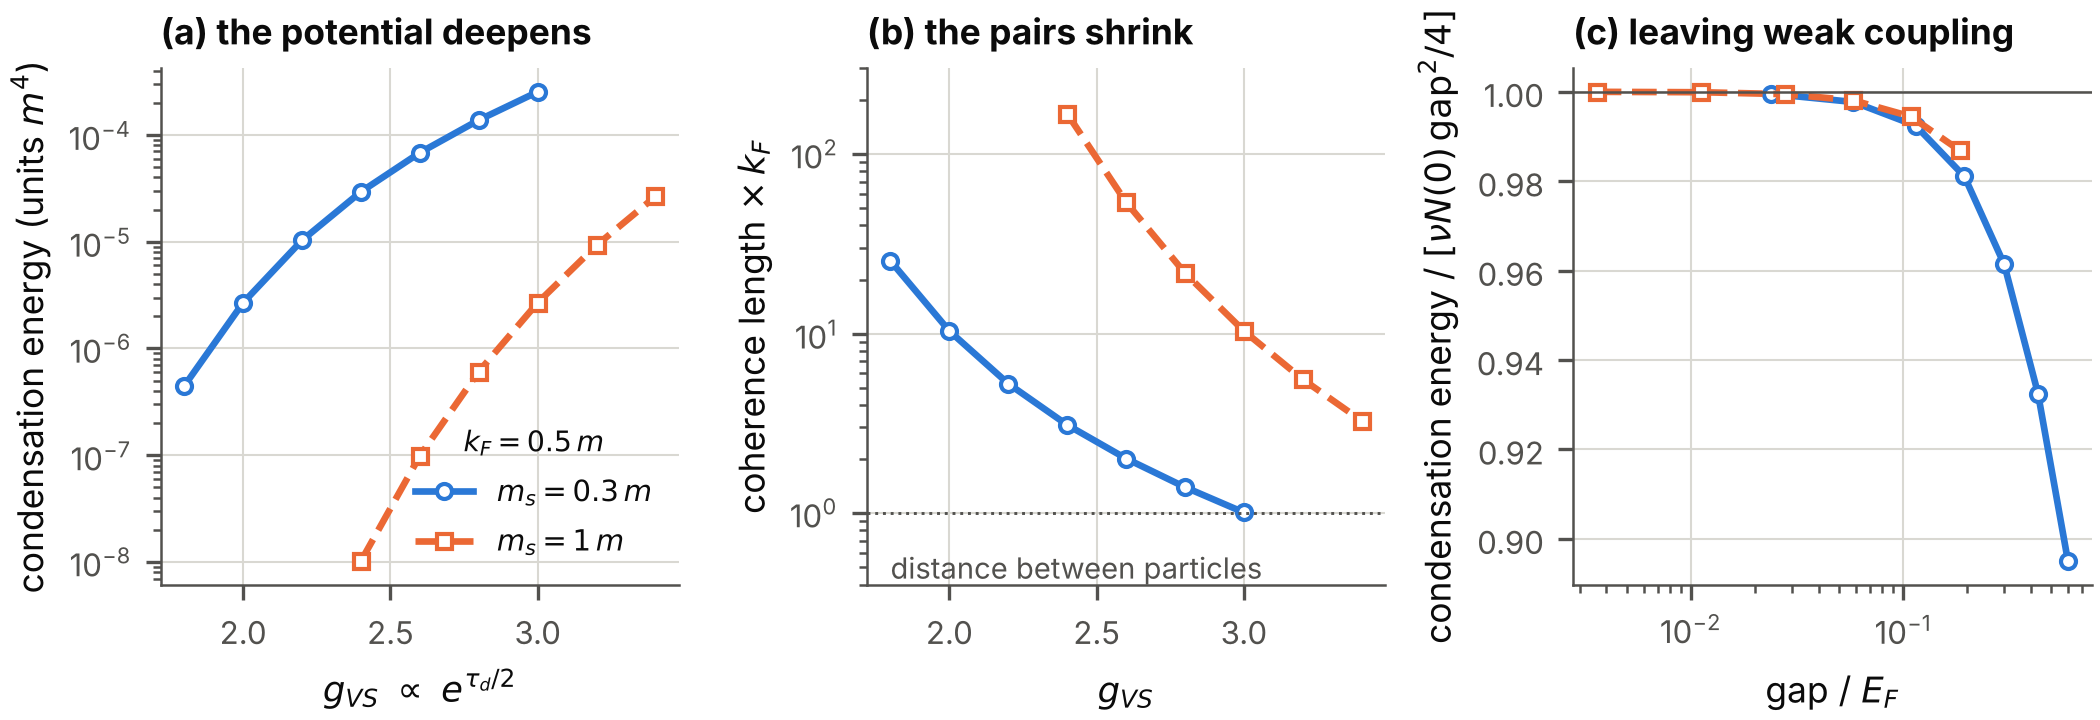
\includegraphics[width=1\textwidth,height=\textheight]{../figures/fig_cjt_history.png}
\caption{The paired state along the clock, from the CJT potential, for
two particles. (a) The condensation energy against the coupling of the
moment. (b) The coherence length of the pair in units of \(1/k_F\). (c)
The condensation energy divided by its weak-coupling value, against the
gap in units of the Fermi kinetic energy: the departure from weak
coupling. Data: \texttt{data/cjt\_history.csv}; program:
\texttt{deflation\ paired}.}
\end{figure}

\hypertarget{thermodynamics}{%
\subsection{2.2 Thermodynamics}\label{thermodynamics}}

At three moments the program follows the paired state of the second
particle from zero temperature to the critical temperature (check
\texttt{def-P2}):

\begin{longtable}[]{@{}
  >{\raggedleft\arraybackslash}p{(\columnwidth - 12\tabcolsep) * \real{0.1429}}
  >{\raggedleft\arraybackslash}p{(\columnwidth - 12\tabcolsep) * \real{0.1429}}
  >{\raggedleft\arraybackslash}p{(\columnwidth - 12\tabcolsep) * \real{0.1429}}
  >{\raggedleft\arraybackslash}p{(\columnwidth - 12\tabcolsep) * \real{0.1429}}
  >{\raggedleft\arraybackslash}p{(\columnwidth - 12\tabcolsep) * \real{0.1429}}
  >{\raggedleft\arraybackslash}p{(\columnwidth - 12\tabcolsep) * \real{0.1429}}
  >{\raggedleft\arraybackslash}p{(\columnwidth - 12\tabcolsep) * \real{0.1429}}@{}}
\toprule\noalign{}
\begin{minipage}[b]{\linewidth}\raggedleft
\(\tau_d\)
\end{minipage} & \begin{minipage}[b]{\linewidth}\raggedleft
\(g_{VS}\)
\end{minipage} & \begin{minipage}[b]{\linewidth}\raggedleft
\(\lambda\)
\end{minipage} & \begin{minipage}[b]{\linewidth}\raggedleft
\(T_c/m\)
\end{minipage} & \begin{minipage}[b]{\linewidth}\raggedleft
\(T_c/E_F\)
\end{minipage} & \begin{minipage}[b]{\linewidth}\raggedleft
gap\((0)/T_c\)
\end{minipage} & \begin{minipage}[b]{\linewidth}\raggedleft
jump of the heat capacity
\end{minipage} \\
\midrule\noalign{}
\endhead
\bottomrule\noalign{}
\endlastfoot
0.000 & 2.60 & 0.156 & \(7.49\times10^{-4}\) & 0.0063 & 1.7640 &
1.4266 \\
0.286 & 3.00 & 0.208 & \(3.90\times10^{-3}\) & 0.0330 & 1.7668 &
1.4331 \\
0.537 & 3.40 & 0.267 & 0.0122 & 0.1036 & 1.7828 & 1.4742 \\
\end{longtable}

While the critical temperature rises by a factor of sixteen, from
\(6.34\times10^{-3}\) to \(1.04\times10^{-1}\) of the Fermi energy, the
ratio of the gap at zero temperature to the critical temperature stays
within 0.019 of the weak-coupling value 1.7639, and the relative jump of
the heat capacity at \(T_c\) within 0.048 of 1.4261. Both ratios are
universal while the coupling is weak; they begin to move at the last
moment, where the gap approaches \(0.2\,E_F\).

\hypertarget{the-ginzburglandau-energy}{%
\subsection{2.3 The Ginzburg--Landau
energy}\label{the-ginzburglandau-energy}}

Near the critical temperature the potential reduces to the
Ginzburg--Landau energy of S1, Sec. 6.2, with three coefficients: the
quadratic coefficient \(a(T)\), the quartic coefficient \(b\) and the
gradient coefficient \(K_{\rm GL}\). The program extracts them from the
CJT potential at the same three moments and compares them with the
weak-coupling formulas (check \texttt{def-P3}):

\begin{longtable}[]{@{}
  >{\raggedleft\arraybackslash}p{(\columnwidth - 14\tabcolsep) * \real{0.1250}}
  >{\raggedleft\arraybackslash}p{(\columnwidth - 14\tabcolsep) * \real{0.1250}}
  >{\raggedleft\arraybackslash}p{(\columnwidth - 14\tabcolsep) * \real{0.1250}}
  >{\raggedleft\arraybackslash}p{(\columnwidth - 14\tabcolsep) * \real{0.1250}}
  >{\raggedleft\arraybackslash}p{(\columnwidth - 14\tabcolsep) * \real{0.1250}}
  >{\raggedleft\arraybackslash}p{(\columnwidth - 14\tabcolsep) * \real{0.1250}}
  >{\raggedleft\arraybackslash}p{(\columnwidth - 14\tabcolsep) * \real{0.1250}}
  >{\raggedleft\arraybackslash}p{(\columnwidth - 14\tabcolsep) * \real{0.1250}}@{}}
\toprule\noalign{}
\begin{minipage}[b]{\linewidth}\raggedleft
\(\tau_d\)
\end{minipage} & \begin{minipage}[b]{\linewidth}\raggedleft
\(g_{VS}\)
\end{minipage} & \begin{minipage}[b]{\linewidth}\raggedleft
\(T_c/m\)
\end{minipage} & \begin{minipage}[b]{\linewidth}\raggedleft
ratio for the slope of \(a(T)\)
\end{minipage} & \begin{minipage}[b]{\linewidth}\raggedleft
ratio for \(b\)
\end{minipage} & \begin{minipage}[b]{\linewidth}\raggedleft
ratio for \(K_{\rm GL}\)
\end{minipage} & \begin{minipage}[b]{\linewidth}\raggedleft
coherence length \(\times\,m\)
\end{minipage} & \begin{minipage}[b]{\linewidth}\raggedleft
coherence length \(\times\,T_c/v_F\)
\end{minipage} \\
\midrule\noalign{}
\endhead
\bottomrule\noalign{}
\endlastfoot
0.000 & 2.60 & \(7.49\times10^{-4}\) & 1.0000 & 1.0001 & 1.0005 & 79.6 &
0.1333 \\
0.286 & 3.00 & \(3.90\times10^{-3}\) & 0.9993 & 0.9949 & 1.0101 & 15.4 &
0.1340 \\
0.537 & 3.40 & 0.0122 & 0.9927 & 0.9641 & 1.0793 & 5.1 & 0.1390 \\
\end{longtable}

(The three columns of ratios are the computed coefficient divided by its
weak-coupling formula.) While \(T_c\) is below \(0.05\,E_F\) the
coefficients agree with the formulas to 1.0 per cent; at the third
moment, \(T_c=0.10\,E_F\), they differ by up to 7.9 per cent. The
consequences of the formulas along the clock are:

\begin{itemize}
\tightlist
\item
  the quadratic coefficient keeps its slope with respect to \(\ln T\),
  which contains the density of states only;
\item
  the quartic and the gradient coefficients fall as \(1/T_c^2\), hence
  as the inverse square of the gap;
\item
  the coherence length of the Ginzburg--Landau energy is
  \(0.1333\,v_F/T_c\) in weak coupling (computed: 0.1333, 0.1340, 0.1390
  at the three moments) and shrinks from 80 to 5.1 in units of \(1/m\).
  \textbf{The cores of the vortices of the superfluid shrink as the
  deflation proceeds.}
\end{itemize}

\hypertarget{the-space-of-the-order-parameter}{%
\subsection{2.4 The space of the order
parameter}\label{the-space-of-the-order-parameter}}

The potential as a function of the direction and of the phase of the
order parameter \(\Delta^a\) is discussed in RS1, Sec. 5.2, with its
table: every unitary state has the potential \(-2\) in units of
\(N(0)\,\mathrm{gap}^2\), with four flat and four positive directions;
the half-paired state has \(-1\); and the deflating axes are not
distinguished from \(x0\) (check \texttt{def-P4}).

\hypertarget{the-bound-pair-from-the-gap-equation}{%
\subsection{2.5 The bound pair, from the gap
equation}\label{the-bound-pair-from-the-gap-equation}}

In vacuum the linearized gap equation is the equation of a bound state
of two fermions. On the deflating spacetime \(D_{VS}=\alpha_{VS}m/m_s\)
grows as \(e^{\tau_d}\) and reaches the value at which the equation has
the eigenvalue 1 at a definite moment (check \texttt{def-P6}):

\begin{longtable}[]{@{}
  >{\raggedleft\arraybackslash}p{(\columnwidth - 6\tabcolsep) * \real{0.2500}}
  >{\raggedleft\arraybackslash}p{(\columnwidth - 6\tabcolsep) * \real{0.2500}}
  >{\raggedleft\arraybackslash}p{(\columnwidth - 6\tabcolsep) * \real{0.2500}}
  >{\raggedleft\arraybackslash}p{(\columnwidth - 6\tabcolsep) * \real{0.2500}}@{}}
\toprule\noalign{}
\begin{minipage}[b]{\linewidth}\raggedleft
\(m_s/m\)
\end{minipage} & \begin{minipage}[b]{\linewidth}\raggedleft
\(D_c\) from the gap equation
\end{minipage} & \begin{minipage}[b]{\linewidth}\raggedleft
\(D_c\) from the Schrödinger equation
\end{minipage} & \begin{minipage}[b]{\linewidth}\raggedleft
difference
\end{minipage} \\
\midrule\noalign{}
\endhead
\bottomrule\noalign{}
\endlastfoot
0.30 & 1.7347 & 1.6798 & 3.3 \% \\
0.10 & 1.6902 & 1.6798 & 0.6 \% \\
0.030 & 1.6810 & 1.6798 & 0.1 \% \\
\end{longtable}

The gap equation has a relativistic kernel, the Schrödinger equation of
RS1, Sec. 4, does not; the two thresholds approach each other as the
radial mode becomes light and the binding non-relativistic.

\begin{center}\rule{0.5\linewidth}{0.5pt}\end{center}

\hypertarget{matter-along-the-clock}{%
\section{3. Matter along the clock}\label{matter-along-the-clock}}

\hypertarget{matter-of-fixed-density-becomes-abnormal}{%
\subsection{3.1 Matter of fixed density becomes
abnormal}\label{matter-of-fixed-density-becomes-abnormal}}

In matter the expectation value \(\phi\) of the Vorton-Scalar is reduced
by the scalar density of the fermions, and with it the fermion mass
\(m^*=g_{VS}\phi\) in the matter. S4, Sec. 5, shows that the reduction
depends on the density and on the single number \(C=g_{VS}^2m^2/m_s^2\),
and that above a critical value of \(C\) the mass vanishes: the matter
is then in the \textbf{abnormal} state, a gas of massless fermions in a
region without expectation value of the scalar. On the deflating
spacetime \(C\propto e^{\tau_d}\) grows at fixed density. The critical
values (check \texttt{def-H5}):

\begin{longtable}[]{@{}
  >{\raggedright\arraybackslash}p{(\columnwidth - 8\tabcolsep) * \real{0.2000}}
  >{\raggedleft\arraybackslash}p{(\columnwidth - 8\tabcolsep) * \real{0.2000}}
  >{\raggedleft\arraybackslash}p{(\columnwidth - 8\tabcolsep) * \real{0.2000}}
  >{\raggedleft\arraybackslash}p{(\columnwidth - 8\tabcolsep) * \real{0.2000}}
  >{\raggedleft\arraybackslash}p{(\columnwidth - 8\tabcolsep) * \real{0.2000}}@{}}
\toprule\noalign{}
\begin{minipage}[b]{\linewidth}\raggedright
Fermi momentum \(k_F/m\)
\end{minipage} & \begin{minipage}[b]{\linewidth}\raggedleft
0.2
\end{minipage} & \begin{minipage}[b]{\linewidth}\raggedleft
0.5
\end{minipage} & \begin{minipage}[b]{\linewidth}\raggedleft
1
\end{minipage} & \begin{minipage}[b]{\linewidth}\raggedleft
2
\end{minipage} \\
\midrule\noalign{}
\endhead
\bottomrule\noalign{}
\endlastfoot
critical \(C\) & 151.892 & 12.971 & 2.556 & 0.617 \\
divided by the estimate \(\pi^2m^2/4k_F^2\) of S4 & 2.46 & 1.31 & 1.04 &
1.00 \\
\end{longtable}

\textbf{Every piece of matter becomes abnormal at a definite moment, the
denser the earlier.} The estimate of the main project is reached at high
density, where the transition happens at weak coupling; at low density
the critical value is larger.

\hypertarget{self-bound-matter}{%
\subsection{3.2 Self-bound matter}\label{self-bound-matter}}

S4 shows that matter is self-bound --- its energy per particle at some
density lies below the mass of a free fermion --- if
\(C>3\pi^2/8=3.7011\) without the filled negative-energy states and if
\(C>3\pi^2/5=5.9218\) with them (check \texttt{def-H1}). Along the clock
(check \texttt{def-P7}; mean field without the negative-energy states,
\(C=4\,e^{\tau_d}\)):

\begin{longtable}[]{@{}
  >{\raggedleft\arraybackslash}p{(\columnwidth - 12\tabcolsep) * \real{0.1429}}
  >{\raggedleft\arraybackslash}p{(\columnwidth - 12\tabcolsep) * \real{0.1429}}
  >{\raggedleft\arraybackslash}p{(\columnwidth - 12\tabcolsep) * \real{0.1429}}
  >{\raggedleft\arraybackslash}p{(\columnwidth - 12\tabcolsep) * \real{0.1429}}
  >{\raggedleft\arraybackslash}p{(\columnwidth - 12\tabcolsep) * \real{0.1429}}
  >{\raggedleft\arraybackslash}p{(\columnwidth - 12\tabcolsep) * \real{0.1429}}
  >{\raggedleft\arraybackslash}p{(\columnwidth - 12\tabcolsep) * \real{0.1429}}@{}}
\toprule\noalign{}
\begin{minipage}[b]{\linewidth}\raggedleft
\(\tau_d\)
\end{minipage} & \begin{minipage}[b]{\linewidth}\raggedleft
\(C\)
\end{minipage} & \begin{minipage}[b]{\linewidth}\raggedleft
energy per particle \(-\,m\) (units \(m\))
\end{minipage} & \begin{minipage}[b]{\linewidth}\raggedleft
\(k_F/m\) at the minimum
\end{minipage} & \begin{minipage}[b]{\linewidth}\raggedleft
\(m^*/m\) there
\end{minipage} & \begin{minipage}[b]{\linewidth}\raggedleft
exchange, radial mode
\end{minipage} & \begin{minipage}[b]{\linewidth}\raggedleft
exchange, phase mode
\end{minipage} \\
\midrule\noalign{}
\endhead
\bottomrule\noalign{}
\endlastfoot
0.00 & 4.00 & -0.0192 & 0.981 & 0.000 & 0.44 \% & 0.51 \% \\
0.25 & 5.14 & -0.0787 & 0.921 & 0.000 & 0.47 \% & 0.54 \% \\
0.50 & 6.59 & -0.1345 & 0.866 & 0.000 & 0.50 \% & 0.59 \% \\
0.75 & 8.47 & -0.1869 & 0.813 & 0.000 & 0.54 \% & 0.66 \% \\
1.00 & 10.87 & -0.2362 & 0.764 & 0.000 & 0.59 \% & 0.73 \% \\
1.25 & 13.96 & -0.2825 & 0.718 & 0.000 & 0.65 \% & 0.82 \% \\
1.50 & 17.93 & -0.3259 & 0.674 & 0.000 & 0.72 \% & 0.93 \% \\
1.75 & 23.02 & -0.3668 & 0.633 & 0.000 & 0.80 \% & 1.06 \% \\
2.00 & 29.56 & -0.4051 & 0.595 & 0.000 & 0.90 \% & 1.22 \% \\
\end{longtable}

Once the threshold is passed, the lowest energy per particle falls
monotonically, from \(-0.0192\,m\) at \(C=4\) to \(-0.405\,m\) at
\(C=29.6\). At every one of these moments the matter of lowest energy is
in the abnormal state, at a Fermi momentum that falls from \(0.98\,m\)
to \(0.59\,m\). The exchange energies of the two modes at that density,
which the mean field omits, are 0.44 and 0.51 per cent of the mean-field
energy at the first moment and 0.90 and 1.22 per cent at the last (for
\(m_s/m=0.3\)): the mean field remains a good approximation along the
whole history.

\emph{Meaning.} On a deflating spacetime, a gas of the fermions of the
model that is dilute and unbound at early times has, at late times, a
state of lower energy: drops of dense abnormal matter, bound by up to 40
per cent of the rest mass at the last moment of the table. Whether and
how fast a gas reaches that state is a question of kinetics that this
supplement does not answer.

\begin{figure}
\centering
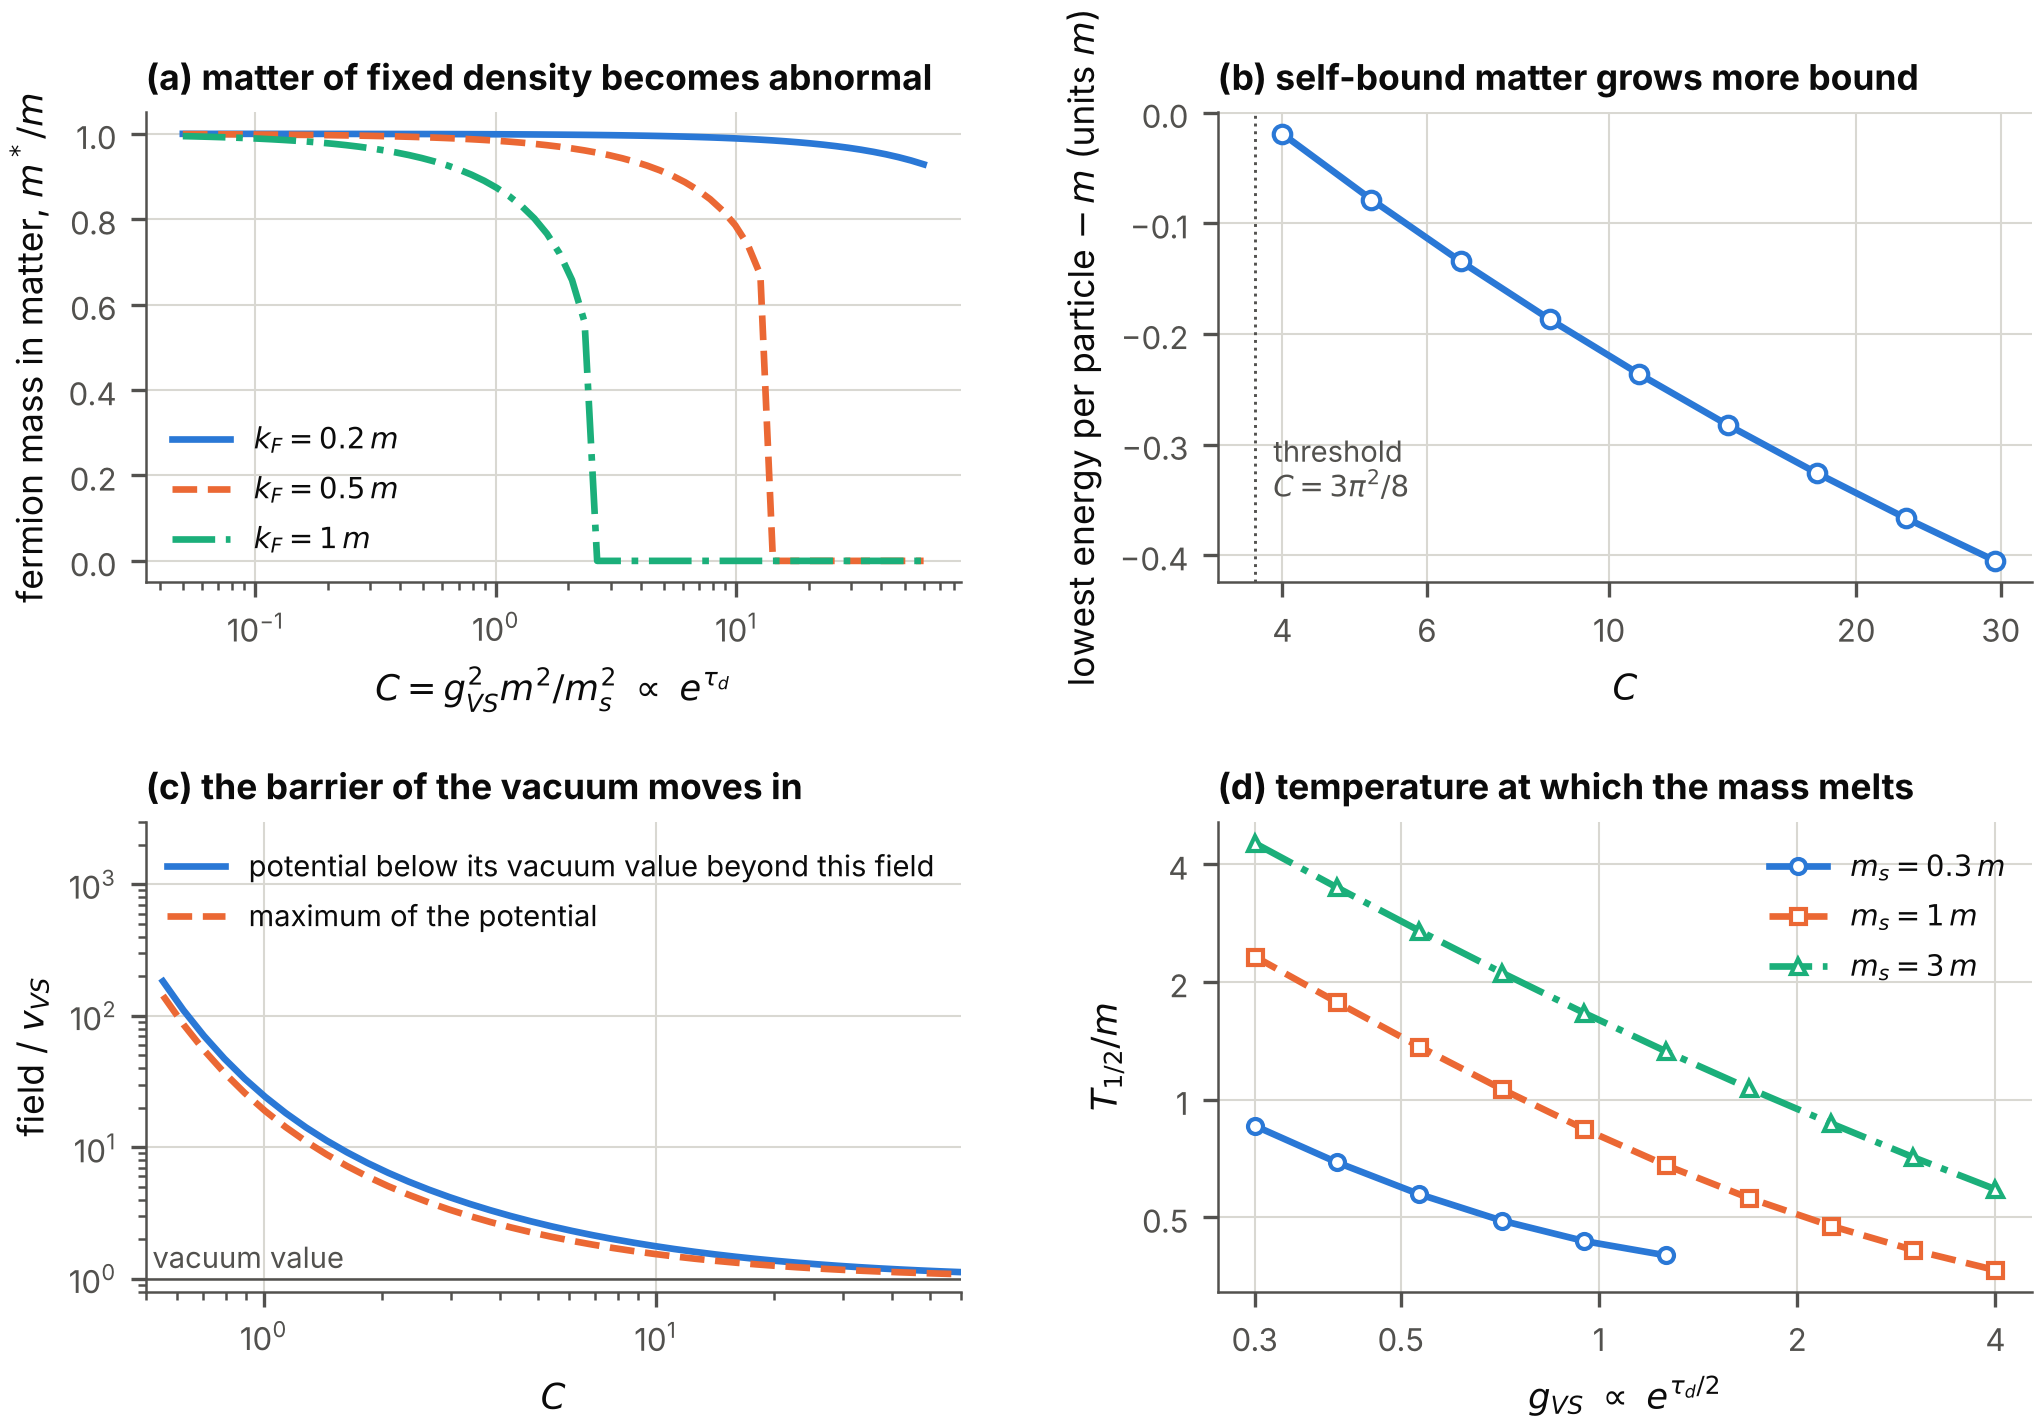
\includegraphics[width=1\textwidth,height=\textheight]{../figures/fig_matter_history.png}
\caption{Matter, vacuum and temperature along the clock. (a) The fermion
mass in matter of three fixed densities against \(C\propto e^{\tau_d}\):
it drops to zero at the critical value. (b) The lowest energy per
particle of self-bound matter, minus \(m\). (c) The field at which the
one-loop potential of the vacuum has its maximum, and the field beyond
which it lies below the vacuum value, in units of the vacuum value. (d)
The temperature at which the fermions have lost half of their mass,
against the coupling, for three ratios \(m_s/m\). Data:
\texttt{data/medium\_history.csv}, \texttt{data/matter\_saturation.csv},
\texttt{data/vacuum\_history.csv}, \texttt{data/thermal\_history.csv};
programs: \texttt{deflation\ history}, \texttt{deflation\ paired}.}
\end{figure}

\begin{center}\rule{0.5\linewidth}{0.5pt}\end{center}

\hypertarget{temperature-the-fermion-mass-melts-earlier-and-earlier}{%
\section{4. Temperature: the fermion mass melts earlier and
earlier}\label{temperature-the-fermion-mass-melts-earlier-and-earlier}}

At high temperature the expectation value of the Vorton-Scalar vanishes
and the fermions are massless (S4, Sec. 6). S4 gives two closed
estimates of the temperature at which this happens and computes, in the
Hartree approximation, the temperatures \(T_{1/2}\) and \(T_0\) at which
the expectation value has fallen to one half and to (nearly) zero. All
are of the order of the four-dimensional vacuum value
\(v_{VS}=m/g_{VS}\), which falls as \(e^{-\tau_d/2}\) while the masses
stay fixed. Along the clock (check \texttt{def-H7}):

\begin{longtable}[]{@{}
  >{\raggedleft\arraybackslash}p{(\columnwidth - 12\tabcolsep) * \real{0.1429}}
  >{\raggedleft\arraybackslash}p{(\columnwidth - 12\tabcolsep) * \real{0.1429}}
  >{\raggedleft\arraybackslash}p{(\columnwidth - 12\tabcolsep) * \real{0.1429}}
  >{\raggedleft\arraybackslash}p{(\columnwidth - 12\tabcolsep) * \real{0.1429}}
  >{\raggedleft\arraybackslash}p{(\columnwidth - 12\tabcolsep) * \real{0.1429}}
  >{\raggedleft\arraybackslash}p{(\columnwidth - 12\tabcolsep) * \real{0.1429}}
  >{\raggedleft\arraybackslash}p{(\columnwidth - 12\tabcolsep) * \real{0.1429}}@{}}
\toprule\noalign{}
\begin{minipage}[b]{\linewidth}\raggedleft
\(m_s/m\)
\end{minipage} & \begin{minipage}[b]{\linewidth}\raggedleft
\(g_{VS}\)
\end{minipage} & \begin{minipage}[b]{\linewidth}\raggedleft
\(C\)
\end{minipage} & \begin{minipage}[b]{\linewidth}\raggedleft
\(T_{\rm high}/m\)
\end{minipage} & \begin{minipage}[b]{\linewidth}\raggedleft
\(T_{1/2}/m\)
\end{minipage} & \begin{minipage}[b]{\linewidth}\raggedleft
\(T_0/m\)
\end{minipage} & \begin{minipage}[b]{\linewidth}\raggedleft
melting defined
\end{minipage} \\
\midrule\noalign{}
\endhead
\bottomrule\noalign{}
\endlastfoot
0.30 & 0.30 & 1.00 & 0.939 & 0.857 & 0.941 & yes \\
0.30 & 0.40 & 1.78 & 0.749 & 0.691 & 0.751 & yes \\
0.30 & 0.53 & 3.16 & 0.617 & 0.573 & 0.618 & yes \\
0.30 & 0.71 & 5.62 & 0.528 & 0.491 & 0.528 & yes \\
0.30 & 0.95 & 10.00 & 0.471 & 0.435 & 0.471 & yes \\
0.30 & 1.26 & 17.8 & 0.436 & 0.400 & 0.436 & yes \\
0.30 & 1.69 & 31.6 & 0.415 & --- & --- & no \\
0.30 & 2.25 & 56.2 & 0.402 & --- & --- & no \\
0.30 & 3.00 & 100.0 & 0.395 & --- & --- & no \\
0.30 & 4.00 & 178 & 0.391 & --- & --- & no \\
1.0 & 0.30 & 0.0900 & 2.605 & 2.325 & 2.627 & yes \\
1.0 & 0.40 & 0.160 & 1.967 & 1.776 & 1.991 & yes \\
1.0 & 0.53 & 0.285 & 1.493 & 1.368 & 1.519 & yes \\
1.0 & 0.71 & 0.506 & 1.143 & 1.065 & 1.170 & yes \\
1.0 & 0.95 & 0.900 & 0.888 & 0.842 & 0.914 & yes \\
1.0 & 1.26 & 1.60 & 0.705 & 0.679 & 0.726 & yes \\
1.0 & 1.69 & 2.85 & 0.577 & 0.561 & 0.587 & yes \\
1.0 & 2.25 & 5.06 & 0.490 & 0.476 & 0.490 & yes \\
1.0 & 3.00 & 9.00 & 0.434 & 0.413 & 0.434 & yes \\
1.0 & 4.00 & 16.0 & 0.399 & 0.366 & 0.399 & yes \\
3.0 & 0.30 & 0.0100 & 4.809 & 4.536 & 4.899 & yes \\
3.0 & 0.40 & 0.0178 & 3.609 & 3.492 & 3.719 & yes \\
3.0 & 0.53 & 0.0316 & 2.710 & 2.707 & 2.842 & yes \\
3.0 & 0.71 & 0.0562 & 2.037 & 2.115 & 2.190 & yes \\
3.0 & 0.95 & 0.1000 & 1.535 & 1.668 & 1.706 & yes \\
3.0 & 1.26 & 0.178 & 1.160 & 1.329 & 1.346 & yes \\
3.0 & 1.69 & 0.316 & 0.881 & 1.070 & 1.075 & yes \\
3.0 & 2.25 & 0.562 & 0.676 & 0.870 & 0.870 & yes \\
3.0 & 3.00 & 1.000 & 0.527 & 0.713 & 0.713 & yes \\
3.0 & 4.00 & 1.78 & 0.420 & 0.590 & 0.590 & yes \\
\end{longtable}

In units of the constant fermion mass, \(T_{1/2}\) falls monotonically
as the coupling grows, for each of the three mass ratios. \textbf{Matter
of a fixed temperature melts at a definite moment of the deflation.}

\emph{A limit of the calculation, stated plainly.} For \(m_s/m=0.3\) no
melting temperature can be given from \(g_{VS}=1.69\) (\(C=32\)) on: the
last four rows of that block. There the one-loop potential of the vacuum
turns over so close to the vacuum value (Sec. 5) that the Hartree
potential ceases to exist at 1.05 times the vacuum value before the
expectation value has fallen. The program marks these moments as not
defined rather than report a number. (An earlier version of the program
reported the artefact of the routine as a temperature; the error is
recorded in the provenance RP9, item R-E14.)

\begin{center}\rule{0.5\linewidth}{0.5pt}\end{center}

\hypertarget{the-vacuum-along-the-clock}{%
\section{5. The vacuum along the
clock}\label{the-vacuum-along-the-clock}}

\hypertarget{the-barrier-moves-in}{%
\subsection{5.1 The barrier moves in}\label{the-barrier-moves-in}}

The one-loop potential of the Vorton-Scalar in vacuum contains the
negative contribution of the fermion loop, which grows with the fourth
power of the field and eventually wins: beyond some field the potential
lies below its value in the vacuum (S4, Sec. 5.3). The larger \(C\), the
smaller that field (check \texttt{def-H6}):

\begin{longtable}[]{@{}
  >{\raggedleft\arraybackslash}p{(\columnwidth - 4\tabcolsep) * \real{0.3333}}
  >{\raggedleft\arraybackslash}p{(\columnwidth - 4\tabcolsep) * \real{0.3333}}
  >{\raggedleft\arraybackslash}p{(\columnwidth - 4\tabcolsep) * \real{0.3333}}@{}}
\toprule\noalign{}
\begin{minipage}[b]{\linewidth}\raggedleft
\(C\)
\end{minipage} & \begin{minipage}[b]{\linewidth}\raggedleft
field at the maximum \(/v_{VS}\)
\end{minipage} & \begin{minipage}[b]{\linewidth}\raggedleft
field beyond which the potential is below its vacuum value \(/v_{VS}\)
\end{minipage} \\
\midrule\noalign{}
\endhead
\bottomrule\noalign{}
\endlastfoot
0.490 & 252 & 324 \\
1.01 & 18.9 & 24.2 \\
9.89 & 1.55 & 1.78 \\
20.3 & 1.25 & 1.37 \\
\end{longtable}

At \(C=1\) the potential falls below its vacuum value only beyond 24.7
times the vacuum value; at \(C=10\) already at 1.77 times. As the
deflation proceeds, the barrier between the vacuum of the model and the
region where the one-loop potential is unbounded below moves in towards
the vacuum.

\emph{What this does and does not mean.} The one-loop potential is not
reliable at fields far from the vacuum value, and a potential that falls
at large field signals that the effective theory needs completion there,
not that the vacuum decays. What the result does establish is a trend:
every statement of the model that rests on the vacuum of the
Vorton-Scalar becomes less secure with time, and beyond \(C\) of order
ten the turning point is within a factor of two of the vacuum value. The
order of this event relative to the binding of the pair depends on
\(m_s/m\) alone and is given in RS1, Sec. 4.2: for \(m_s/m<4.9\) the
potential has fallen below its vacuum value at three times the vacuum
value \emph{before} two fermions bind.

\hypertarget{a-pair-condensate-in-the-vacuum}{%
\subsection{5.2 A pair condensate in the
vacuum}\label{a-pair-condensate-in-the-vacuum}}

S4, Sec. 7, asks whether the pair can condense without a medium, and
finds from the ladder equation with a momentum cutoff that this requires
\(\alpha_{VS}\) above a critical value of order one. With the cutoff
\(100\,m\) the critical values are between 2.13 and 2.93 for the six
mass ratios of RS1, Sec. 4.2. On the deflating spacetime \(\alpha_{VS}\)
reaches such a value at a definite moment --- but at that moment the
coupling is strong, the one-boson exchange is no longer a controlled
approximation, and by Sec. 5.1 the vacuum of the model is no longer
protected. The statement of S4 stands, with one addition: a pair
condensate in the vacuum is not reached by the deflation within the
range of validity of the model.

\begin{center}\rule{0.5\linewidth}{0.5pt}\end{center}

\hypertarget{what-has-been-established-and-what-has-not}{%
\section{6. What has been established, and what has
not}\label{what-has-been-established-and-what-has-not}}

\textbf{Established.}

\begin{enumerate}
\def\labelenumi{\arabic{enumi}.}
\tightlist
\item
  Along the deflation clock the solution of the gap equation is a
  minimum of the CJT potential at every moment examined; its
  condensation energy, critical temperature, thermodynamic ratios,
  Ginzburg--Landau coefficients and coherence lengths are given in Sec.
  2, with their weak-coupling laws and the moments at which these fail.
\item
  Matter of fixed density becomes abnormal at a critical value of \(C\)
  that the deflation reaches at a definite time (Sec. 3.1); matter is
  self-bound for \(C>3.7011\) and more strongly bound later (Sec. 3.2).
\item
  The melting temperature of the fermion mass falls along the clock
  (Sec. 4).
\item
  The barrier of the one-loop vacuum potential moves towards the vacuum
  value (Sec. 5.1).
\end{enumerate}

\textbf{Not established.}

\begin{enumerate}
\def\labelenumi{\arabic{enumi}.}
\tightlist
\item
  \emph{Strong coupling.} Every history ends in a regime that the
  two-loop truncation does not control. The numbers at the last moments
  of each table indicate the trend; they are not predictions.
\item
  \emph{Kinetics.} The sections give sequences of equilibrium states.
  Only for the paired state has the ability to follow been examined
  (RS1, Sec. 7). How a gas reaches the self-bound state, and whether the
  abnormal state forms by nucleation, are open.
\item
  \emph{The vacuum beyond one loop.} Sec. 5.1 uses the one-loop
  potential outside its range of reliability, as S4 does, and draws only
  the conclusion stated there.
\item
  \emph{The neglected term.} The shift of the boson masses by
  \(\mathrm{gsum}^2/4\) is neglected throughout (Sec. 1). It would
  matter only for a rate of deflation comparable with a particle mass.
\end{enumerate}

\begin{center}\rule{0.5\linewidth}{0.5pt}\end{center}

\hypertarget{appendix-a.-complete-output-of-the-programs}{%
\section{Appendix A. Complete output of the
programs}\label{appendix-a.-complete-output-of-the-programs}}

\hypertarget{a.1-deflation-paired}{%
\subsection{\texorpdfstring{A.1
\texttt{deflation\ paired}}{A.1 deflation paired}}\label{a.1-deflation-paired}}

\begin{Shaded}
\begin{Highlighting}[]
\NormalTok{PROJECT spacetimes, Revision\_Deflation: the results of the CJT effective action along the deflation clock}
\NormalTok{generated by: deflation (Rust crate spacetimes{-}deflation, version 0.1.0; PROJECT spacetimes, Revision\_Deflation); command: deflation paired}
\NormalTok{7 of 7 checks passed}

\NormalTok{[PASS] def{-}P1  (numerical) the paired state along the clock (13 moments, two particles): at every moment the solution of the gap equation is a minimum of the CJT potential (Newton\textquotesingle{}s method on the potential reproduces the iterated gap function to 7.7e{-}12; the minimum along the ray lies at s = 1 to 4.6e{-}7; the smallest eigenvalue of the second variation is positive), the critical temperature from the potential equals that of the linearized gap equation to 2.6e{-}12, and the condensation energy is within 15 per cent of {-}nu N(0) gap\^{}2/4 wherever the gap is below 0.1 E\_F. The condensation energy deepens monotonically, in weak coupling with twice the logarithmic slope of the gap (to within 0.1 per cent), and the coherence length of the pair shrinks: for the first particle from 25 to 1.0 in units of 1/k\_F. At the last 5 moments of that particle the gap exceeds 0.1 E\_F, and at the last one the coherence length has fallen to the distance 1/k\_F between the particles: the deflation carries the paired state from overlapping pairs towards bound pairs}
\NormalTok{[PASS] def{-}P2  (numerical) thermodynamics along the clock: while the critical temperature rises from 6.34e{-}3 to 1.04e{-}1 E\_F (g\_VS = 2.6 to 3.4), the ratio gap(0)/T\_c stays within 0.019 of the weak{-}coupling value 1.7639 and the jump of the heat capacity within 0.048 of 1.4261: both ratios are universal while the coupling is weak, and they move only slightly as the gap approaches 0.2 E\_F at the last moment}
\NormalTok{[PASS] def{-}P3  (numerical) Ginzburg{-}Landau energy along the clock (three moments, T\_c = 6.3e{-}3, 3.3e{-}2, 1.0e{-}1 E\_F): while T\_c is below 0.05 E\_F the coefficients from the CJT potential agree with the weak{-}coupling formulas to 1.0 per cent; at the third moment, T\_c = 0.10 E\_F, they differ by up to 7.9 per cent, the state leaving the weak{-}coupling regime. The quadratic coefficient keeps its slope 4 N(0), the quartic and the gradient coefficients fall as 1/T\_c\^{}2, and the coherence length, sqrt(7 zeta(3)/(48 pi\^{}2)) v\_F/T\_c = 0.1333 v\_F/T\_c in weak coupling (computed: 0.1333, 0.1340, 0.1390), shrinks from 80 to 5.1 (units 1/m). Vortex cores shrink as the deflation proceeds}
\NormalTok{[PASS] def{-}P4  (numerical) the space of the order parameter on the deflating spacetimes (frame components along x0, x5, x6, x7; both spacetimes): every unitary state, whichever its direction, has all eight gaps equal and the potential {-}2 (units of N(0) gap\^{}2), with four flat directions (the Goldstone modes) and four directions of positive curvature; the half{-}paired state has four gaps closed and the potential {-}1. The potential does not distinguish the deflating axes from x0: in this sector the deflation selects no direction of the order parameter}
\NormalTok{[PASS] def{-}P5  (numerical) the test of the CJT method on the zero{-}dimensional model, executed again: the two{-}loop truncation, the one used for the models, has a solution for every coupling from 0.01 to 30 and stays within 10.7 per cent of the exact propagator}
\NormalTok{[PASS] def{-}P6  (numerical) the moment of binding from the gap equation: the linearized gap equation in vacuum reaches the eigenvalue 1 at D\_VS = 1.7347, 1.6902, 1.6810 for m\_s/m = 0.3, 0.1, 0.03, approaching the value 1.67981 of the Schroedinger equation as the binding becomes non{-}relativistic (relative differences 3.3e{-}2, 6.2e{-}3, 6.9e{-}4)}
\NormalTok{[PASS] def{-}P7  (numerical) self{-}bound matter along the clock: once C has passed 3.7011 the lowest energy per particle lies below m, and it falls monotonically as the deflation proceeds: from {-}0.0192 m at C = 4 to {-}0.405 m at C = 29.6. At every one of these moments the matter of lowest energy is in the abnormal state (fermion mass zero inside the matter, largest value of m*/m in the table 0.0e0), at a Fermi momentum that falls from 0.98 m to 0.59 m. The exchange energies of the radial and of the phase mode at that density are 0.44 and 0.51 per cent of the mean{-}field energy at C = 4, and 0.90 and 1.22 per cent at C = 29.6 (m\_s/m = 0.3): the mean field remains a good approximation along the whole history}
\NormalTok{[PASS] ALL  (numerical) every check above passed}
\end{Highlighting}
\end{Shaded}

\hypertarget{a.2-deflation-history}{%
\subsection{\texorpdfstring{A.2
\texttt{deflation\ history}}{A.2 deflation history}}\label{a.2-deflation-history}}

\begin{Shaded}
\begin{Highlighting}[]
\NormalTok{PROJECT spacetimes, Revision\_Deflation: checks of the history of the model along the deflation clock (couplings that grow as exp(gsum x4))}
\NormalTok{generated by: deflation (Rust crate spacetimes{-}deflation, version 0.1.0; PROJECT spacetimes, Revision\_Deflation); command: deflation history}
\NormalTok{8 of 8 checks passed}

\NormalTok{[PASS] def{-}H1  (numerical) thresholds of the model, computed again: a pair of fermions is bound if D\_VS \textgreater{} 1.67981; matter is self{-}bound if C \textgreater{} 3.7011 (3 pi\^{}2/8 = 3.7011) or, with the negative{-}energy states, C \textgreater{} 5.9218 (3 pi\^{}2/5 = 5.9218). On a deflating spacetime D\_VS and C grow as exp(gsum x4), so each threshold is passed at a definite x4}
\NormalTok{[PASS] def{-}H2  (numerical) along the clock, wherever the gap is below 0.05 E\_F the critical temperature is 0.567 times the gap (largest deviation 0.0020); the gap of the vector channel is at every moment at least as large as the gap with the radial mode alone, and that at least as large as the gap of the two{-}form channel; the gap never decreases as the deflation proceeds (four sets of m\_s/m and k\_F/m, 34 moments each)}
\NormalTok{[PASS] def{-}H3  (numerical) growth of the gap: for a weakly coupled state the gap is proportional to exp({-}1/lambda), where lambda = lambda\_S + lambda\_P is the sum of the pairing strengths of the radial mode and of the phase mode in the vector channel, and lambda grows as exp(tau\_d), which gives d ln(gap)/d tau\_d = 1/lambda; in the computed histories lambda d ln(gap)/d tau\_d lies between 1.00 and 1.03 wherever 1e{-}6 \textless{} gap/E\_F \textless{} 0.02: the gap grows much faster than the couplings, by one e{-}folding in the time 1/(gsum/lambda)}
\NormalTok{[PASS] def{-}H4  (numerical) the moment at which a pair becomes bound: just below D\_c the scattering length is large and negative ({-}134.0/m\_s at 0.99 D\_c), just above large and positive (135.9/m\_s at 1.01 D\_c); the binding energy starts as a power of the distance from the threshold with the exponents 2.01 (between 2 and 4 per cent above D\_c) and 2.01 (between 4 and 8 per cent), that is quadratically: E\_b \textasciitilde{} (exp(tau\_pair) {-} 1)\^{}2 m\_s\^{}2/m. Because E\_b vanishes at the threshold, the pair cannot follow the deflation adiabatically at first, however slow the deflation is}
\NormalTok{[PASS] def{-}H5  (numerical) matter of fixed density loses the fermion mass (the Vorton{-}Scalar loses its expectation value in the matter) when C passes a critical value that falls with the density: k\_F = 0.2 m: C = 151.892 (2.46 times pi\^{}2 m\^{}2/(4 k\_F\^{}2)); k\_F = 0.5 m: C = 12.971 (1.31 times pi\^{}2 m\^{}2/(4 k\_F\^{}2)); k\_F = 1 m: C = 2.556 (1.04 times pi\^{}2 m\^{}2/(4 k\_F\^{}2)); k\_F = 2 m: C = 0.617 (1.00 times pi\^{}2 m\^{}2/(4 k\_F\^{}2)). The estimate C = pi\^{}2 m\^{}2/(4 k\_F\^{}2) of the main project is reached at high density, where the transition happens at weak coupling; at low density the critical C is larger. On a deflating spacetime every piece of matter becomes abnormal at a definite x4, the denser the earlier}
\NormalTok{[PASS] def{-}H6  (numerical) the field beyond which the one{-}loop potential of the Vorton{-}Scalar lies below its vacuum value decreases monotonically as C grows: 24.7 v\_VS at C = 1, 1.77 v\_VS at C = 10. As the deflation proceeds the barrier that protects the vacuum moves in towards the vacuum value}
\NormalTok{[PASS] def{-}H7  (numerical) the temperature T\_half at which the fermions lose half of their mass, in units of the (constant) fermion mass, falls monotonically as g\_VS grows, for m\_s/m = 0.3, 1 and 3 (26 of the 30 moments examined; it is of the order of the four{-}dimensional vacuum value m/g\_VS, which falls as exp({-}gsum x4/2)): matter of a fixed temperature melts at a definite x4. No melting temperature can be given for m\_s/m = 0.3 from g\_VS = 1.69 (C = 32) on; there the Hartree potential ceases to exist at 1.05 v\_VS before the expectation value has fallen, because the one{-}loop potential turns over too close to the vacuum value}
\NormalTok{[PASS] def{-}H8  (numerical) order of events: the pair of fermions becomes bound before the one{-}loop potential of the Vorton{-}Scalar has fallen below its vacuum value at a field of 3 v\_VS only for the mass ratios m\_s/m = 10, 30 of the six ratios 0.1, 0.3, 1, 3, 10, 30 examined (the condition is 4 pi D\_c m/m\_s \textless{} 4.27, i.e. m\_s/m \textgreater{} 4.9): for a light radial mode the deflation destabilizes the vacuum first}
\NormalTok{[PASS] ALL  (numerical) every check above passed}
\end{Highlighting}
\end{Shaded}

\hypertarget{appendix-b.-files}{%
\section{Appendix B. Files}\label{appendix-b.-files}}

\begin{longtable}[]{@{}
  >{\raggedright\arraybackslash}p{(\columnwidth - 4\tabcolsep) * \real{0.1905}}
  >{\raggedright\arraybackslash}p{(\columnwidth - 4\tabcolsep) * \real{0.6190}}
  >{\raggedright\arraybackslash}p{(\columnwidth - 4\tabcolsep) * \real{0.1905}}@{}}
\toprule\noalign{}
\begin{minipage}[b]{\linewidth}\raggedright
file
\end{minipage} & \begin{minipage}[b]{\linewidth}\raggedright
content
\end{minipage} & \begin{minipage}[b]{\linewidth}\raggedright
written by
\end{minipage} \\
\midrule\noalign{}
\endhead
\bottomrule\noalign{}
\endlastfoot
\texttt{code/deflation-rs/src/cmd\_paired.rs} & the paired state along
the clock from the CJT potential of the main project & --- \\
\texttt{code/deflation-rs/src/history.rs} & matter, vacuum and
temperature along the clock & --- \\
\texttt{data/cjt\_history.csv} & Sec. 2.1 &
\texttt{deflation\ paired} \\
\texttt{data/cjt\_thermo\_history.csv},
\texttt{data/cjt\_gl\_history.csv} & Secs. 2.2 and 2.3 &
\texttt{deflation\ paired} \\
\texttt{data/order\_parameter\_states.csv} & Sec. 2.4 &
\texttt{deflation\ paired} \\
\texttt{data/cjt\_toy.csv}, \texttt{data/cjt\_threshold.csv} & Sec. 1
(test of the method) and Sec. 2.5 & \texttt{deflation\ paired} \\
\texttt{data/matter\_saturation.csv} & Sec. 3.2 &
\texttt{deflation\ paired} \\
\texttt{data/medium\_history.csv} & Sec. 3.1 &
\texttt{deflation\ history} \\
\texttt{data/thermal\_history.csv} & Sec. 4 &
\texttt{deflation\ history} \\
\texttt{data/vacuum\_history.csv}, \texttt{data/events.csv} & Sec. 5 &
\texttt{deflation\ history} \\
\texttt{data/paired\_checks.txt}, \texttt{data/history\_checks.txt} (and
\texttt{.csv}) & Appendix A & the two commands \\
\texttt{figures/fig\_cjt\_history},
\texttt{figures/fig\_matter\_history} (\texttt{.pdf}, \texttt{.png}) &
the two figures & \texttt{make\_figures.py} \\
\end{longtable}

\end{document}
